\chapter{Methodology}\label{chapter:methodology}

\begin{figure}
	\centering
	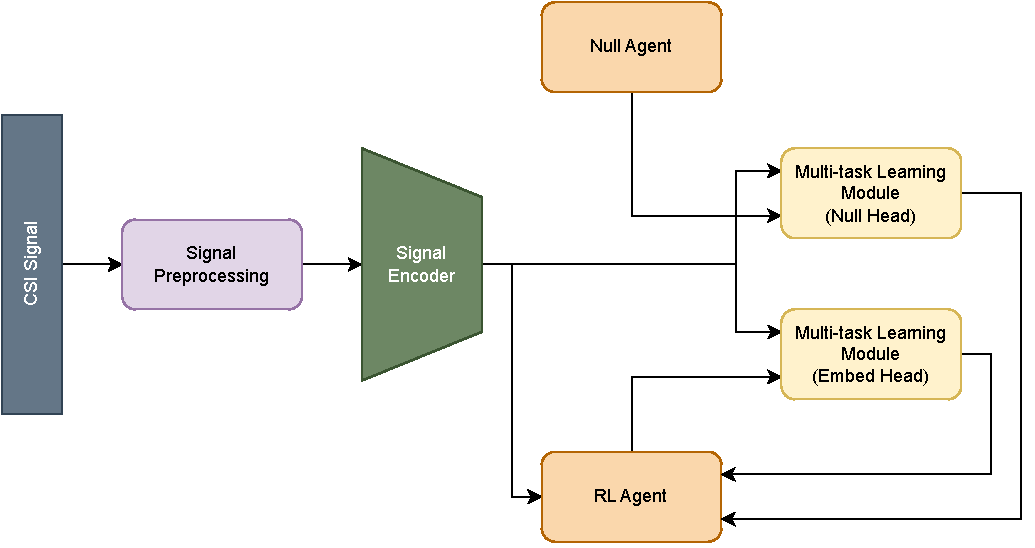
\includegraphics[width=\linewidth]{figures/arch_diagram.pdf}
	\caption{An abstracted diagram of the proposed DARLInG architecture.}
	\label{fig:arch-diagram}
\end{figure}

This chapter will first discuss the details of the dataset which we are using. 
We will discuss our approach to the problem of domain agnostic Wi-Fi CSI gesture classification and delve into the details of our chosen architecture.
This will first begin with a general overview of our method, then discuss each component of the architecture individually as well as their motivations and intuitions.

\section{Widar 3.0}
DO THIS

\section{DARLInG}

In this thesis, we present our novel approach DARLInG (Domain Autolabeling through Reinforcement Learning for the Identification of Gestures).
DARLInG is our proposed approach to domain-agnostic gesture identification using RL.
Our intuition comes from \cite{zhang2021adversarial} in which RL was used to identify features in the data which was invariant to domain shifts.
Analogously, we hypothesize that RL can then be used to identify those features which are \textit{not} invariant to domain shifts and produce a \textit{domain embedding} from said features.
We hypothesize that by providing our gesture discriminator with not only the original signal, encoded by a VAE-style encoder, but also this domain embedding, the gesture discriminator would be able to significantly increase its performance in gesture recognition throughout multiple domains.

The general architecture of DARLInG can be seen in Figure \ref{fig:arch-diagram}.
We first propose a signal preprocessing and signal-to-image transformation pipeline, described in Section \ref{sec:methodology-signal-preprocessing} and \ref{sec:methodology-signal-to-image}.
This transforms the input signal into an image that is then passed through a CNN encoder, as described in Section \ref{sec:methodology-signal-encoding}, encoding the signal into a latent space.
This latent representation is then used in two different ways: As an input for the multi-task learning heads, described in Section \ref{sec:methodology-multi-task-learning}, and as the state observation for our RL agent, described in Section \ref{sec:methodology-rl}.

\begin{figure}
	\centering
	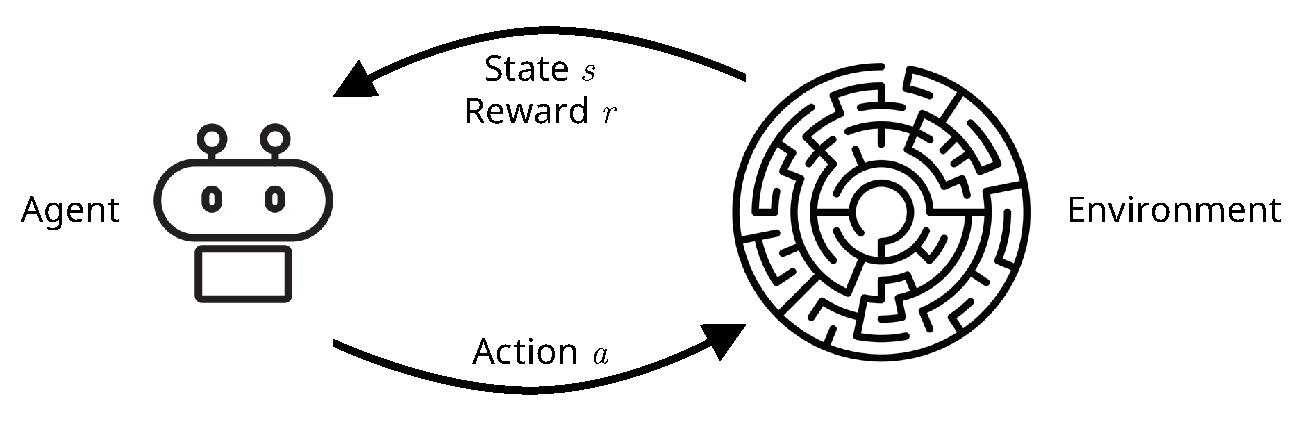
\includegraphics[width=0.78\textwidth]{figures/rl_paradigm}
	\caption{The basic paradigm of Reinforcement Learning where an agent interacts with its environment through actions $a$ and receives a new state $s$ and reward $r$ in return.}\label{fig:rl-paradigm}
\end{figure}
Recall first that RL is typically modeled as a Markov decision process with an environment and observed state of that environment at time $t$, $s_t$. An agent then performs an action $a_t$ and is provided with a reward $r_t$ and a new observed state $s_{t+1}$.
A typical RL scenario is framed in this way and is visually represented by Figure \ref{fig:rl-paradigm}.

To mitigate domain-shift, our RL agent is tasked with producing the best possible domain embedding of the domain $\boldsymbol{d}_r = a, \boldsymbol{d}_r \in [0, 1]^e$ as its action where $e$ is the dimensionality of the domain embedding.
The domain embedding, or action, is generated by the RL agent given the signal latent representation $\boldsymbol{z} = s, \boldsymbol{z} \in [0, 1]^f$ as its state observation, where $f$ is the dimensionality of the latent representation.

To provide the RL agent with a reward function, inspired by triplet loss, we use two different multi-task learning modules.
The details of the reward function are described in Subsection \ref{subsec:methodology-reward}.
One of these modules is provided $\boldsymbol{d}_{\emptyset}$, representing a vector of zeros when the $d$ is one-hot encoded or a value of $\frac{1}{f}$ when $\boldsymbol{d}_r$ is a probability measure, and the other $\boldsymbol{d}_{r}$.

%\todonotestodo[inline]{This chapter is not finalized, due to the possibility of changing things around so will be kept as bullet points at this stage.}

\section{Signal Preprocessing}\label{sec:methodology-signal-preprocessing}

\begin{figure}
	\centering
	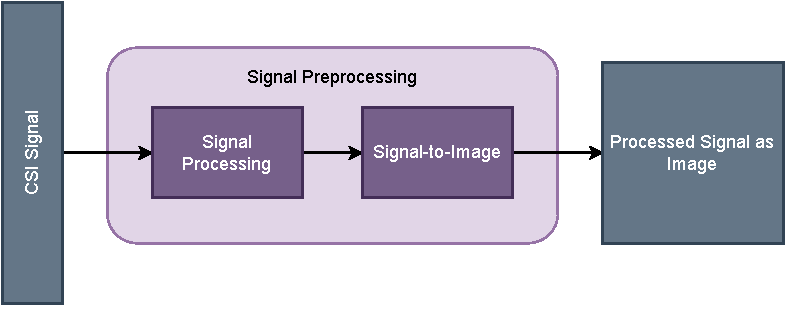
\includegraphics[width=0.8\linewidth]{figures/signal_preprocessing_diagram.pdf}
	\caption{Details of the signal preprocessing module. The module is comprised of traditional signal preprocessing and a signal-to-image transformation.}
	\label{fig:signal-preprocessing-diagram}
\end{figure}

As the old adage goes, garbage in, garbage out.
As such, we propose a signal preprocessing module, visualized in Figure \ref{fig:signal-preprocessing-diagram}.
This module first cleans the CSI signal using traditional signal processing and then transforms it into an image for use by the signal encoder.

\subsection{Signal Processing}

\begin{figure}
	\centering
	\begin{subfigure}{0.49\textwidth}
		\centering
		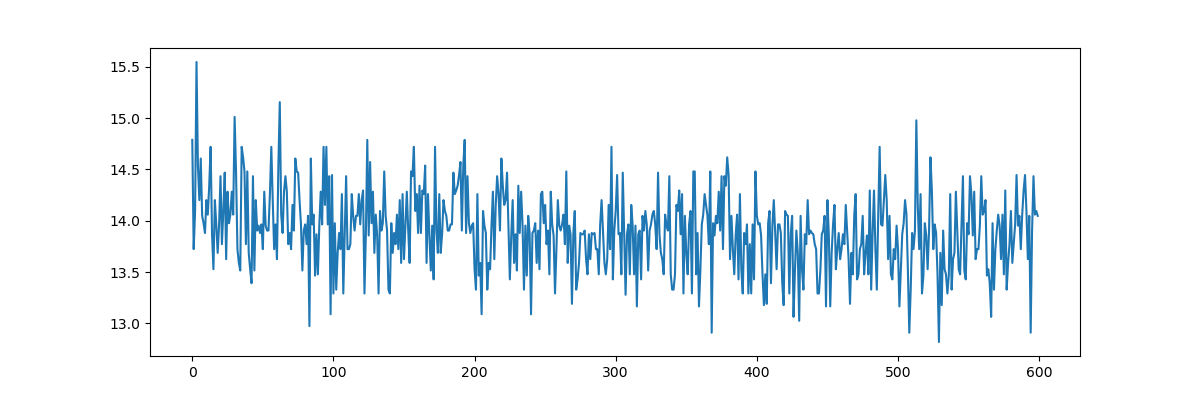
\includegraphics[width=\textwidth]{figures/amp_original}
		\caption{The original amplitude signal.}
	\end{subfigure}
	\hfill
	\begin{subfigure}{0.49\textwidth}
		\centering
		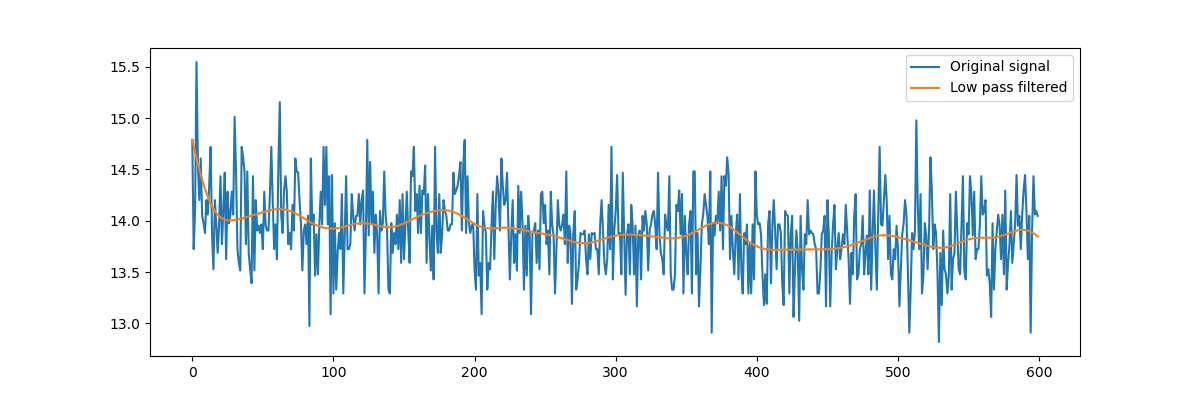
\includegraphics[width=\textwidth]{figures/amp_step_1}
		\caption{The original amplitude signal and the low pass filtered signal.}
	\end{subfigure}
	\hfill
	\begin{subfigure}{0.49\textwidth}
		\centering
		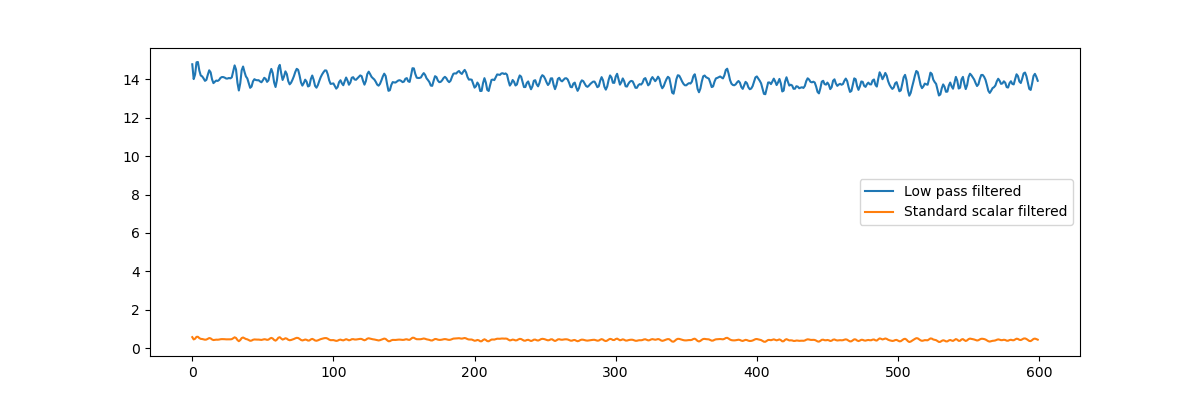
\includegraphics[width=\textwidth]{figures/amp_step_2}
		\caption{The low pass filtered signal and the signal after the standard scalar.}
	\end{subfigure}
	\hfill
	\caption{An example of the amplitude shift signal after being transformed by each step of the signal processing pipeline. Only the first 600 samples of one channel from one tranceiver link is shown here for illustrative purposes.} \label{fig:amp-pipeline}
\end{figure}

\begin{figure}
	\centering
	\begin{subfigure}{0.49\textwidth}
		\centering
		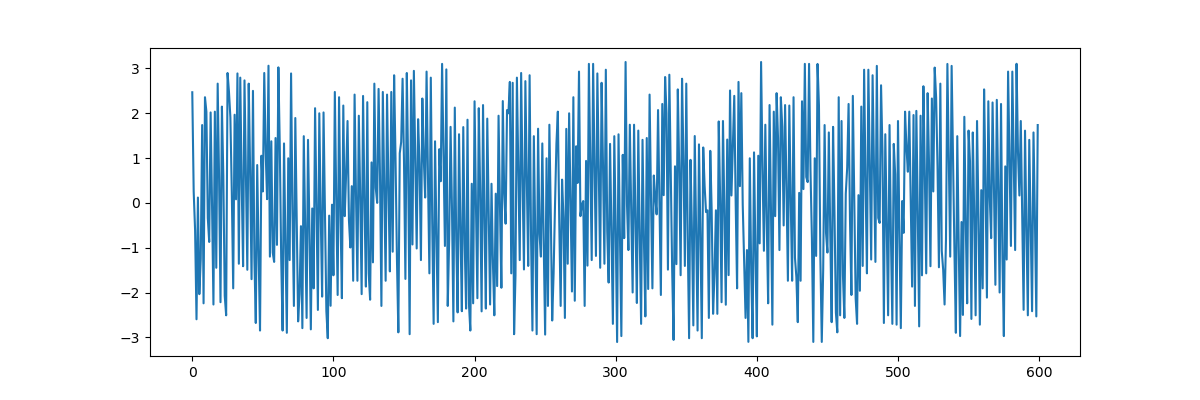
\includegraphics[width=\textwidth]{figures/phase_original}
		\caption{The original phase signal.}
	\end{subfigure}
	\hfill
	\begin{subfigure}{0.49\textwidth}
		\centering
		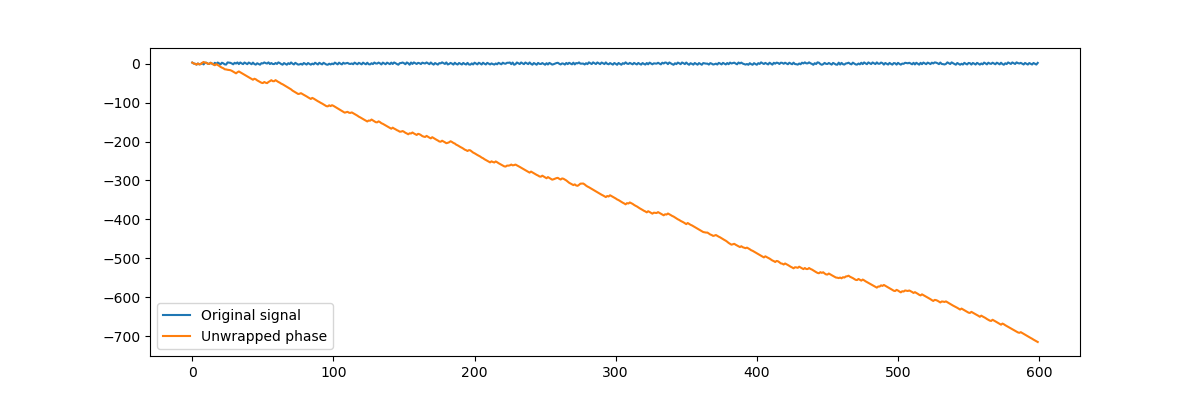
\includegraphics[width=\textwidth]{figures/phase_step_1}
		\caption{The original phase signal and the phase unwrapped signal.}
	\end{subfigure}
	\hfill
	\begin{subfigure}{0.49\textwidth}
		\centering
		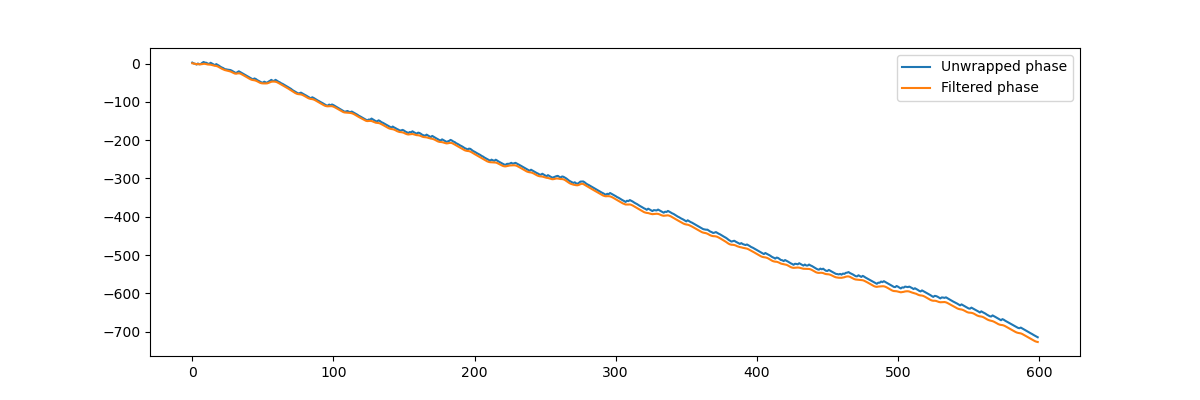
\includegraphics[width=\textwidth]{figures/phase_step_2}
		\caption{The phase unwrapped signal and the phase filtered signal.}
	\end{subfigure}
	\hfill
	\begin{subfigure}{0.49\textwidth}
		\centering
		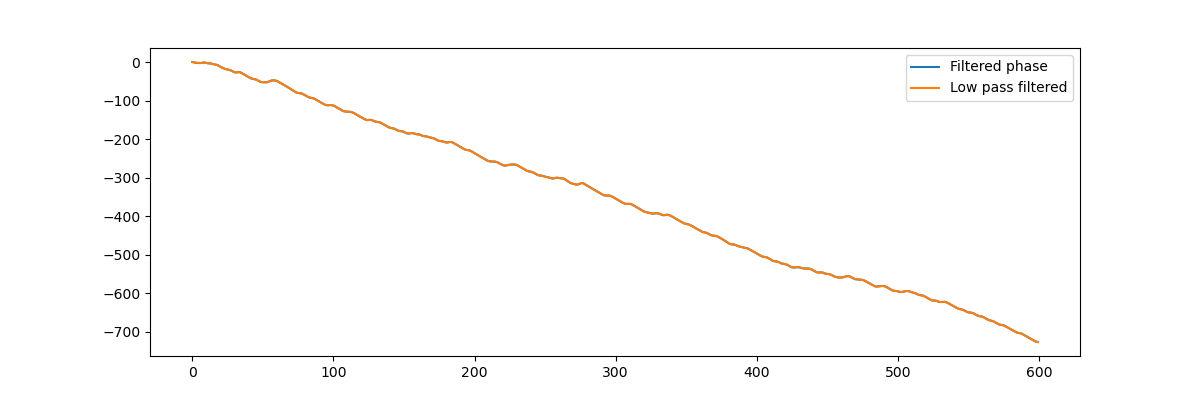
\includegraphics[width=\textwidth]{figures/phase_step_3}
		\caption{The phase filtered signal and the low pass filtered signal.}
	\end{subfigure}
	\hfill
	\begin{subfigure}{0.49\textwidth}
		\centering
		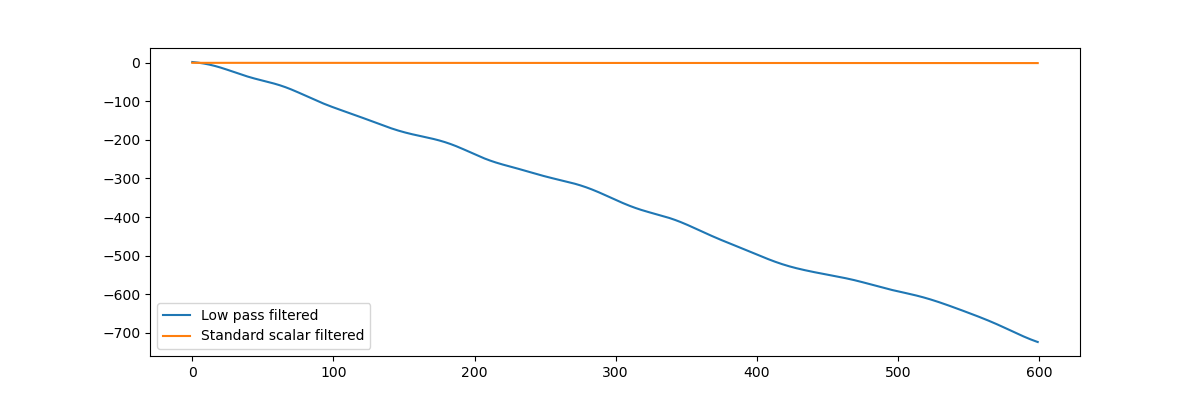
\includegraphics[width=\textwidth]{figures/phase_step_4}
		\caption{The low pass filtered signal and the signal after the standard scalar.}
	\end{subfigure}
	\hfill
	\caption{An example of the phase shift signal after being transformed by each step of the signal processing pipeline. Only the first 600 samples of one channel from one tranceiver link is shown here for illustrative purposes.} \label{fig:phase-pipeline}
\end{figure}

\begin{figure}
	\centering
	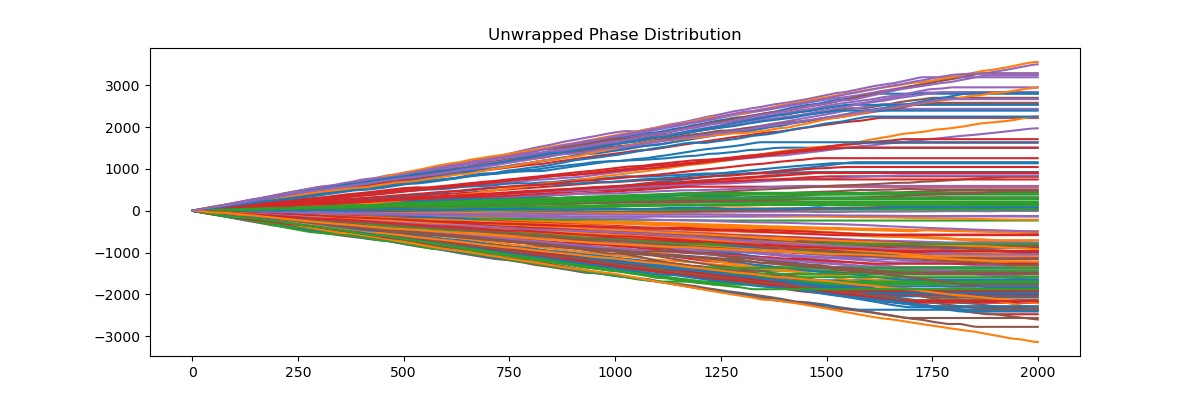
\includegraphics[width=0.8\textwidth]{figures/phase_unwrap}
	\caption{A plot over time of the phase shift after unwrapping of all training data, colored by gesture, showing how there is no general trend of only increasing or decreasing phases.}\label{fig:phase-unwrap}
\end{figure}

The CSI data is provided as a set of complex values sampled at 1000 Hz.
We first decompose this into its radius and angle components on the complex plane or its amplitude and phase shifts, respectively.
We process this signal through two different pipelines, one for the amplitude component and one for the phase component, as the phase requires a few additional processing steps compared to the amplitude.

The pipeline for amplitude consists of the following steps:

\begin{enumerate}
	\item \textbf{Low Pass Filter} set to a cutoff frequency of 25 Hz and an order of 4.
	\item \textbf{Standard Scalar} which has been trained on all training data and transforms the signal to have a mean of 0 and a standard deviation of 1.
\end{enumerate}

The low pass filter is used to eliminate noise inherent in CSI data from environmental factors.
It has also been set to these values based on empirical experimentation which shows that no human movements during the performance of the 6 gestures which we test for has a frequency above 250 Hz.

The standard scalar is used since empirical evidence shows that neural networks work best when input values are close to the interval $[-1, 1]$ \cite{varun2023tuning}.

The effect of each step of the amplitude pipeline can be seen in Figure \ref{fig:amp-pipeline}.

The pipeline for the phase consists of the following steps prepended to the amplitude pipeline:
\begin{enumerate}
	\item \textbf{Phase Unwrapping} which unwraps the phase and makes the signal continuous.
	\item \textbf{Phase Filtering} step, which applies a uniform and median filter onto the phase shift signal, inspired by \cite{oerlemans2022effect}.
\end{enumerate}

The effect of each step of the phase pipeline can be seen in Figure \ref{fig:phase-pipeline}.

The signal can now be considered clean, or at least clean enough that we can continue with further steps.

During the course of experimentation, we considered taking the derivative of the phase, to eliminate a generally monotonously increasing or decreasing signal, as can been seen in the example in \ref{fig:phase-pipeline} after phase unwrapping.
Further investigation showed that this is actually not necessary as most signals do not monotonously increase or decrease.
A plot of the phase shifts after unwrapping of all signals can be seen in Figure \ref{fig:phase-unwrap}.
The plot clearly shows that there is no general trend of phases increasing or decreasing infinitely, with many phase shifts staying around 0 after unwrapping.

\subsection{Signal-to-Image Transformation}\label{sec:methodology-signal-to-image}

%Four crazy signal-to-image transformation methods! You won't believe number three!\todo{If there are no objections, this will be in the final paper}

The next stage in our method is transform the signal into an image, leveraging advances from computer vision.
There are many works from the literature which show that there are certainly improvements that can be gained from performing image processing on temporal data.
We will experiment with the following four methods for signal-to-image transformation: Gramian Angular Fields (GAF) \cite{wang2015imaging}, Markov Transition Fields (MTF) \cite{wang2015imaging}, and Recurrent Plots (RP) \cite{eckmann1995recurrence}.

Regardless of the chosen method, the signal has now been transformed into an image and we can proceed with the encoding of this image into a latent space.

\section{Signal encoding}\label{sec:methodology-signal-encoding}

The encoding of the signal, now an image, into a latent space is performed using CNN-based image processing methods.

\begin{itemize}
	\item The signal encoding backbone is a standard CNN
	\item This will probably be something simple, like ResNet since the signal shouldn't be too complex that it requires something very SOTA
	\item Alternatively, mobilenet may be used as well
	\item This may actually be the least important aspect of this thesis
\end{itemize}

The latent representation of this signal is then passed to both the reinforcement learning agent as its state observation as well as to the multi-task learning modules.
How the RL agent uses this state observation is described in Section \ref{sec:methodology-rl} while its use by the multi-task learning module is described in Section \ref{sec:methodology-multi-task-learning}.

\section{Unsupervised Domain Representations through Reinforcement Learning}\label{sec:methodology-rl}

\subsection{Reward Function}\label{subsec:methodology-reward}
To mitigate domain shift, we implement a novel method for unsupervised domain representations through reinforcement learning.

\begin{itemize}
	\item Base terminology: Agent, action, state observation (state), and reward
	\item The encoder-decoder architecture described in Section \ref{sec:methodology-signal-encoding} and \ref{sec:methodology-multi-task-learning} is the environment.
	\item RL loop:
	\begin{enumerate}
		\item The agent receives the image embedding produced by the encoder/backbone as its state
		\item The reinforcement learning agent produces an embedding of the domain as its action
		\item The environment is trained with one pair of heads receiving the action of the agent while the other pair receives senseless values (either all 0s if the representation is one-hot or a uniform distribution if the representation is a probability measure)
		\item After training of the agent, the RL agent is provided a reward from the environment which is used to improve the agent
	\end{enumerate}
	\item Let a performance metric function $M$ denote the gesture classification performance of a multi-task learning module given the gesture classification prediction $\hat{y_{c}}$. Then, the reward function $R$ of the agent is $R\left(M\left(\hat{y}_{c,rl}, y_c\right),M\left(\hat{y}_{c,0}, y_c\right)\right)$ and calculates the gesture prediction performance difference between the module given the domain embedding and the module given the null embedding.
	\begin{itemize}
		\item The intuition is, the reward is based on how much better the head pair with the action should perform than the head pair without the action
		\item This is based on the idea behind triplet loss, where in an unsupervised scenario, model performance can be determined by the metric performance differential between two inputs. Maximizing this difference implies better total model performance.
		\item We will also experiment with L1 vs L2 regularization on the reward, representated by the function $R$.
	\end{itemize}
	\item To speed up training, we take a page from AutoML competitions and the environment is trained within 1 minute and be focused on improving performance as fast as possible instead of achieving the best performance, at least during hyperparam optimization
	\item After hyperparameters are chosen, then we train properly and fully.
	\item A reward is then calculated using the function $R\left(M\left(\hat{y}_{rl}, y\right)-M\left(\hat{y}_{0}, y\right)\right)$, where $M$ is the metric used to calculate the performance of the gesture classifier in each multi-task learning module and $R$ is some reward function.
	\item We do not use the absolute difference, as we are interested in the having negative values representing the module provided $D_0$ having better performance.
	\item We will be looking at PPO \cite{schulman2017proximal} and SARSA \cite{rummery1994line}
	\begin{itemize}
		\item We've used both these techniques before in a previous project, so implementation should be relatively straightforwards
	\end{itemize}
	\item \emph{Motivation}
	\begin{itemize}
		\item We use the RL agent inspired by \cite{ma2021location} and hypothesize that the RL architecture there can be extended to domain auto-labeling
		\item We use the triplet-loss approach since triplet loss is a proven way to provide a numerical value showing the difference between two input
		\begin{itemize}
			\item In other words, this is analogous to testing the null hypothesis, where $H_0$ is no RL agent produced domain embedding and $H_1$ is a RL agent produced domain embedding
			\item Our hypothesis is that the domain embedding will produce better results
			\item If the RL agent can be trained, then the difference $(M\left(\hat{y}_{rl}, y\right)-M\left(\hat{y}_{0}, y\right)$ will approach $M\left(\hat{y}_{rl}, y\right)$ producing the maximum reward for the RL agent
		\end{itemize}
	\end{itemize}
\end{itemize}

\section{Multi-task Learning}\label{sec:methodology-multi-task-learning}

\begin{figure}
	\centering
	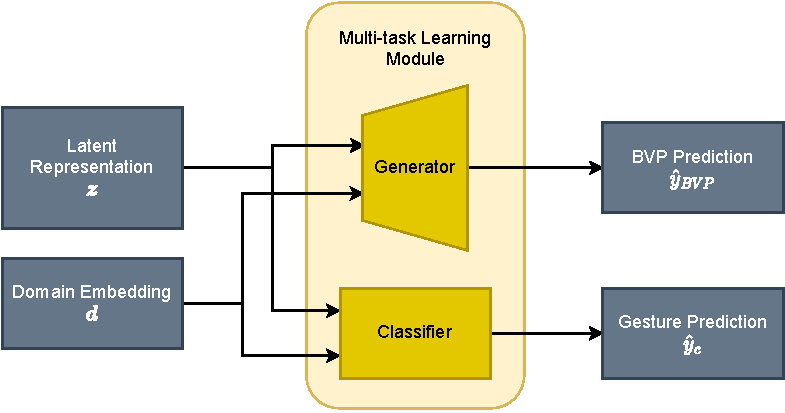
\includegraphics[width=0.8\linewidth]{figures/multitask_learning_module_diagram.pdf}
	\caption{Details of the multi-task learning module. The generator is made up of a series of deconvolutional layers and produces the BVP prediction while the classifier is a fully connected network and produces a probability distribution over each gesture class.}
	\label{fig:multitask-learning-module-diagram}
\end{figure}

The actual gesture classification module is built using a multi-task learning module, a visualization of which can be seen in Figure \ref{fig:multitask-learning-module-diagram}.

\begin{itemize}
	\item The idea is to enforce some sort of representation that \textit{can} be used to get a domain-independent representation of the data
	\item We utilize multi-task learning for this, where one head is used to predict BVP, which is theoretically domain-independent \cite{zheng2019zero}
	\begin{itemize}
		\item We are not actually interested in the BVP, but having it as part of our training will enforce the need for a representation which is theoretically domain-independent.
		\item \cite{martini2021domain} suggests the use of MMD and an adversarial approach to training the model to ensure that while the representation is domain-invariant, it still retains enough discriminatory powers such that the domain classifier can still perform.
		\item Instead of this approach, we use the BVP prediction to enforce a representation which is domain-invariant and we use an RL agent instead of the domain classifier suggested in \cite{martini2021domain}.
	\end{itemize}
	\item The other head is a classifier head and classifies gestures
	\item It's been shown that doing multi-task learning like this leads to good results with latent representations which are more robust \cite{tuggener2021deepscoresv2}
	\item We duplicate this pair of heads to enable a reward function for the RL agent inspired by triplet loss
	\item Loss function for the gesture classifier is cross entropy loss
	\item Loss function for the BVP generator is cross entropy loss on the produced image.
	\item \emph{Motivation}
	\begin{itemize}
		\item We use multi-task learning since its been shown that multitask learning can produce better/more powerful/more robust/more efficient latent representations due to the latent representation being used for multiple tasks
		\item For this multi-task objective, we use BVP as the target of the generator, since we have ground-truth BVP data and \cite{zheng2019zero} makes a point to show that BVP is domain-independent
		\begin{itemize}
			\item Therfore, if the generator can produce a BVP close to the ground-truth, then we have a latent representation that can be used to produce domain-independent features
		\end{itemize}
		\item We want try to get a latent representation capable of producing domain-independent features but we don't want to enforce it directly on the latent representation, since this may not work well \cite{van2022insights} and \cite{martini2021domain} suggests giving the representation some discriminatory abilities w.r.t. the domain.
		\begin{itemize}
			\item Therefore, we believe that enforcing domain independence on the output will result in a representation that is domain-independent enough yet still retain discriminatory power.
		\end{itemize}
		\item Cross Entropy loss on the produced image is used since it is the appropriate loss function for image generation (i.e., pixel-wise feature value prediction)
		\item We use gesture as the target of the classifier, since that's the goal of this thesis
		\item Cross Entropy loss on the prediction is used since it is the appropriate loss function for a multi-class prediction task.
		
	\end{itemize}
\end{itemize}
